\documentclass[a4paper,11pt]{article}
\usepackage{amsmath,amsthm,amsfonts,amssymb,bm} 
\usepackage{graphicx,psfrag} 
\usepackage{fancyhdr}
\usepackage{color} 
\usepackage{geometry}
\usepackage{multirow}
\usepackage{listings}
\usepackage{enumerate}
\usepackage{leftidx} 
\usepackage{mathrsfs} 
\usepackage{xeCJK}

\usepackage{listings}
\usepackage{color}
\usepackage{fontspec}
\setmainfont{Helvetica}
\definecolor{mygreen}{rgb}{0,0.6,0}
\definecolor{mygray}{rgb}{0.5,0.5,0.5}
\definecolor{mymauve}{rgb}{0.58,0,0.82}

\lstset{ %
  backgroundcolor=\color{white},   % choose the background color; you must add \usepackage{color} or \usepackage{xcolor}
  basicstyle=\footnotesize,        % the size of the fonts that are used for the code
  breakatwhitespace=false,         % sets if automatic breaks should only happen at whitespace
  breaklines=true,                 % sets automatic line breaking
  captionpos=b,                    % sets the caption-position to bottom
  commentstyle=\color{mygreen},    % comment style
  deletekeywords={...},            % if you want to delete keywords from the given language
  escapeinside={\%*}{*)},          % if you want to add LaTeX within your code
  extendedchars=true,              % lets you use non-ASCII characters; for 8-bits encodings only, does not work with UTF-8
  keepspaces=true,                 % keeps spaces in text, useful for keeping indentation of code (possibly needs columns=flexible)
  keywordstyle=\bfseries,       % keyword style
  language=SQL,                 % the language of the code
  morekeywords={*,...},            % if you want to add more keywords to the set
  numbers=none,                    % where to put the line-numbers; possible values are (none, left, right)
  numbersep=5pt,                   % how far the line-numbers are from the code
  numberstyle=\tiny\color{mygray}, % the style that is used for the line-numbers
  rulecolor=\color{black},         % if not set, the frame-color may be changed on line-breaks within not-black text (e.g. comments (green here))
  showspaces=false,                % show spaces everywhere adding particular underscores; it overrides 'showstringspaces'
  showstringspaces=false,          % underline spaces within strings only
  showtabs=false,                  % show tabs within strings adding particular underscores
  stepnumber=2,                    % the step between two line-numbers. If it's 1, each line will be numbered
  stringstyle=\color{mymauve},     % string literal style
  tabsize=2,                       % sets default tabsize to 2 spaces
  title=\lstname                   % show the filename of files included with \lstinputlisting; also try caption instead of title
}

\setCJKmainfont{Kai}
\geometry{left=3.17cm,right=3.17cm,top=2.54cm,bottom=2.54cm}

\begin{document}

\pagestyle{fancy}
\rfoot{\thepage}
\rhead{\bfseries Database System Concept}
\setlength{\parskip}{0.7ex plus0.2ex minus0.2ex}
\cfoot{\empty}
\lhead{\empty}


\title{Assignment 4}
\author{Qinglin Li, 5110309074}
\date{}
\maketitle

\headheight 3pt
\thispagestyle{fancy}

\section*{Problem 1}
\begin{itemize}
\item \textbf{Super key} is a set of attributes that uniquely identifies a tuple within a relation,
\item \textbf{Candidate key} is a super key and no proper subset of it can be a super key. 
\item \textbf{Primary key} is the candidate key that is selected to identify tuples uniquely within the relation.
\end{itemize}

\section*{Problem 2}
\begin{itemize}
\item \textbf{Weak entity set} is an entity set has no sufficient attributes to form a primary key.
\item \textbf{Strong entity set} is an entity set has a primary key. 
\end{itemize}

\section*{Problem 3}
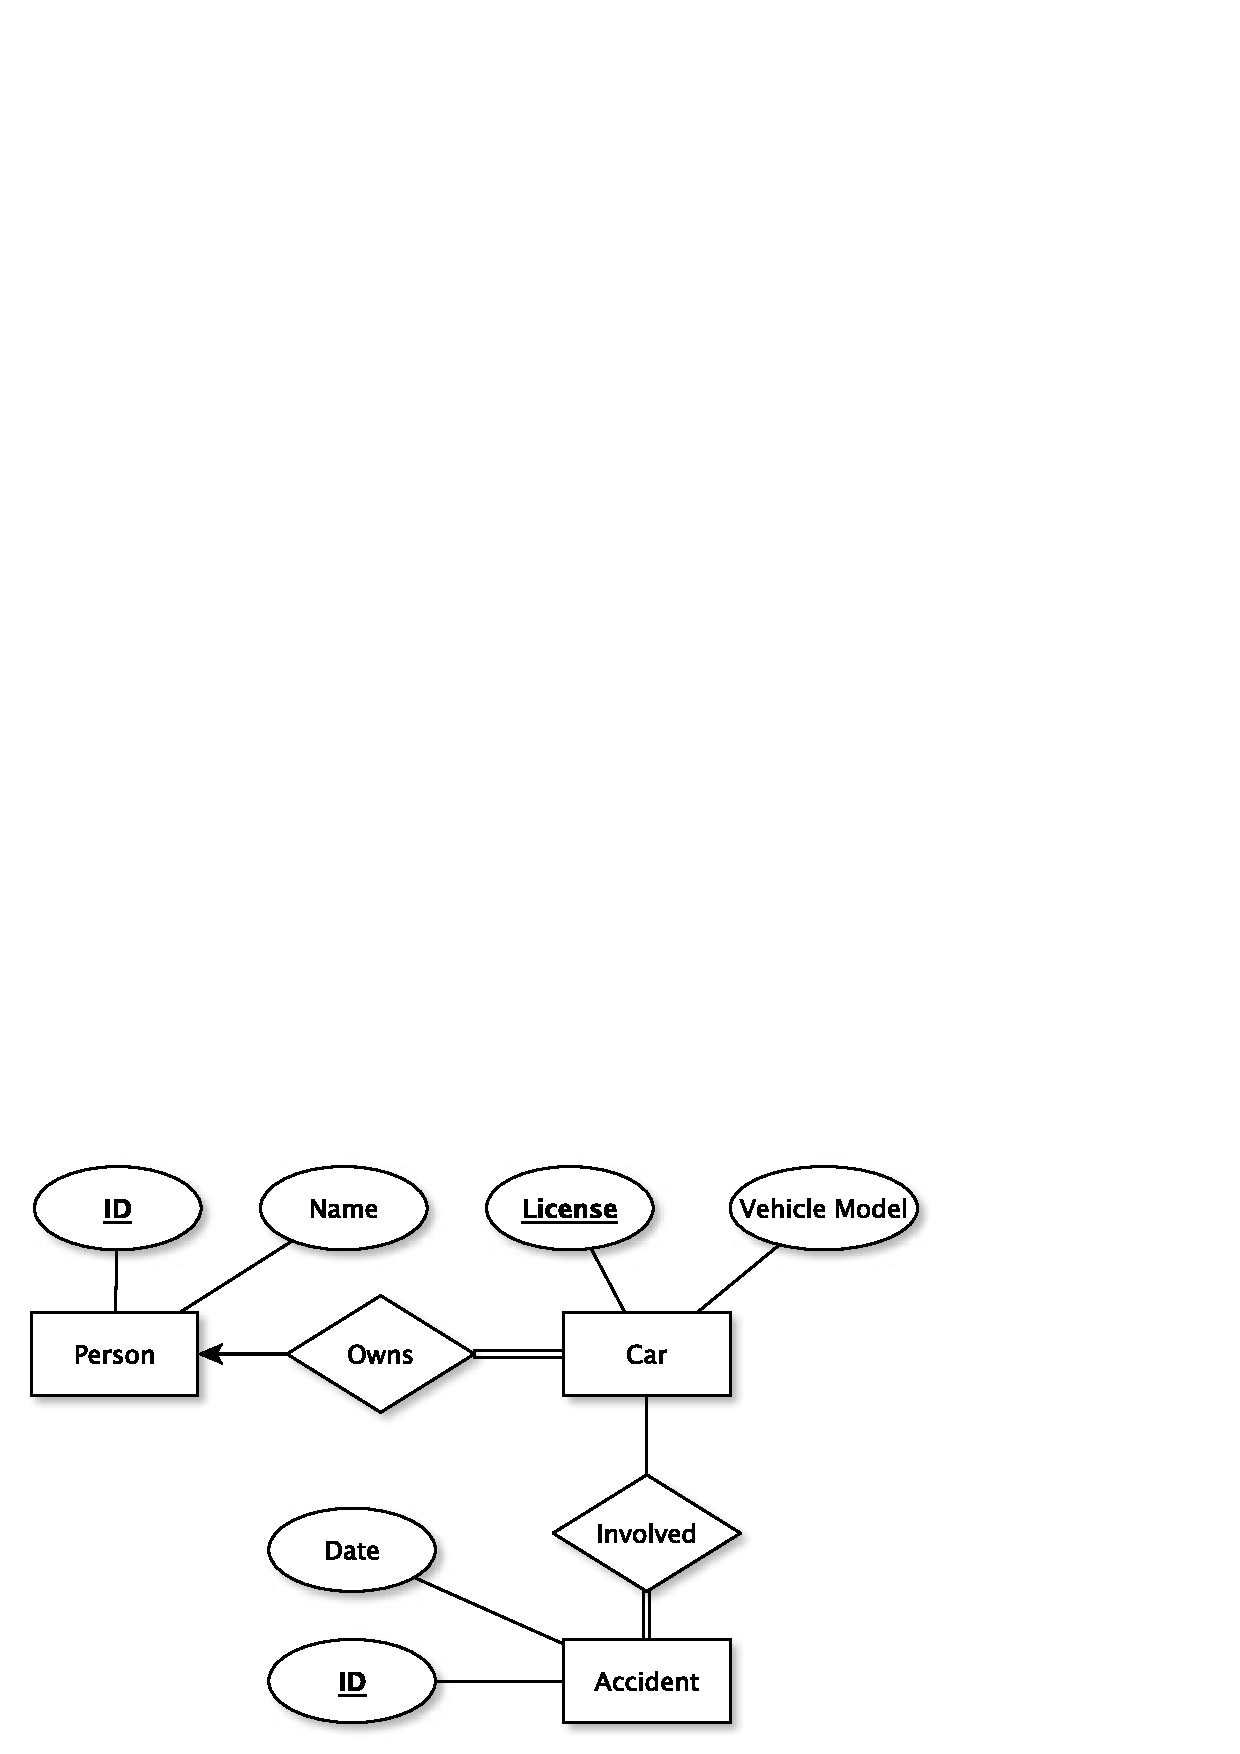
\includegraphics{p3.pdf}

\section*{Problem 4}
\begin{enumerate}[a)]
\item
\includegraphics[scale=0.4]{p4a}
\item 
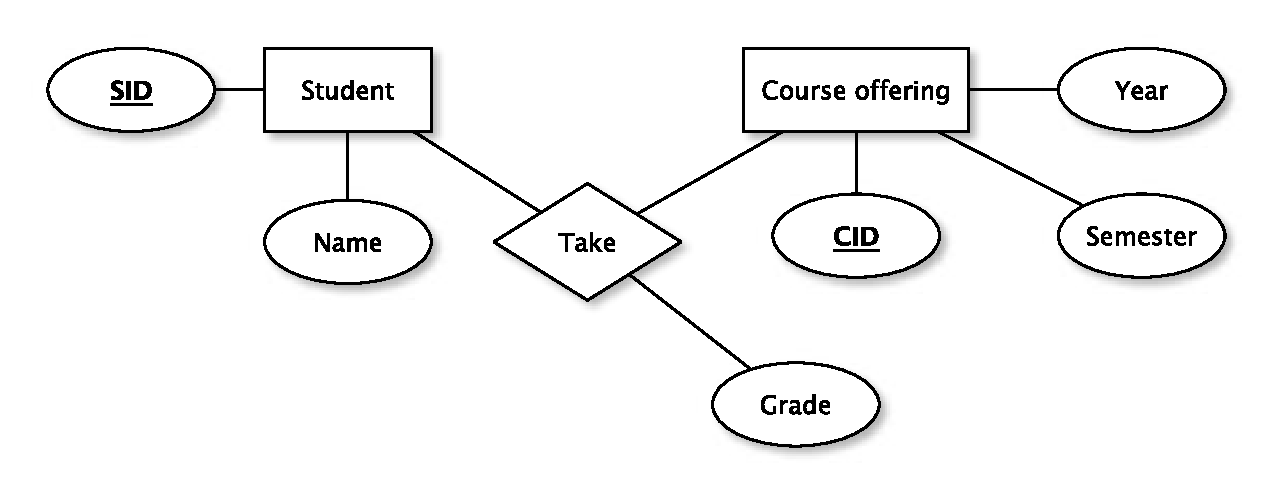
\includegraphics[scale=0.4]{p4b}
\end{enumerate}

\section*{Problem 5}
\begin{lstlisting}
create table person(
	ID int primary key not null auto_increment,
	name varchar(20)
);

create table car(
	license varchar(20) primary key not null,
	person_id int references person,
	vehicle_model varchar(20) not null
);

create table accident(
	ID int primary key not null auto_increment,
	accident_date date not null
);

create table involved(
	accident_id int references accident,
	car_license varchar(20) references car,
	primary key (accident_id, car_license)
);
\end{lstlisting}

\section*{Problem 6}
\textbf{Aggregation} is an abstraction through which relationships are treated as higher-level entities. Thus the relationship between entities can be treated as an entity.\\

Examples:
\begin{enumerate}
\item Programmers work for projects. A programmer works for a certain project using many languages.
\item Workers work for projects. A worker work for a centain project using many tools.
\end{enumerate}
\end{document}
